\clearpage
%We hypothesize that our approximation yields more accurate solutions because SGD operates on inexact gradients and our approximate formulation handles them better.

\begin{minipage}{\textwidth}
%\begin{figure}[th]
%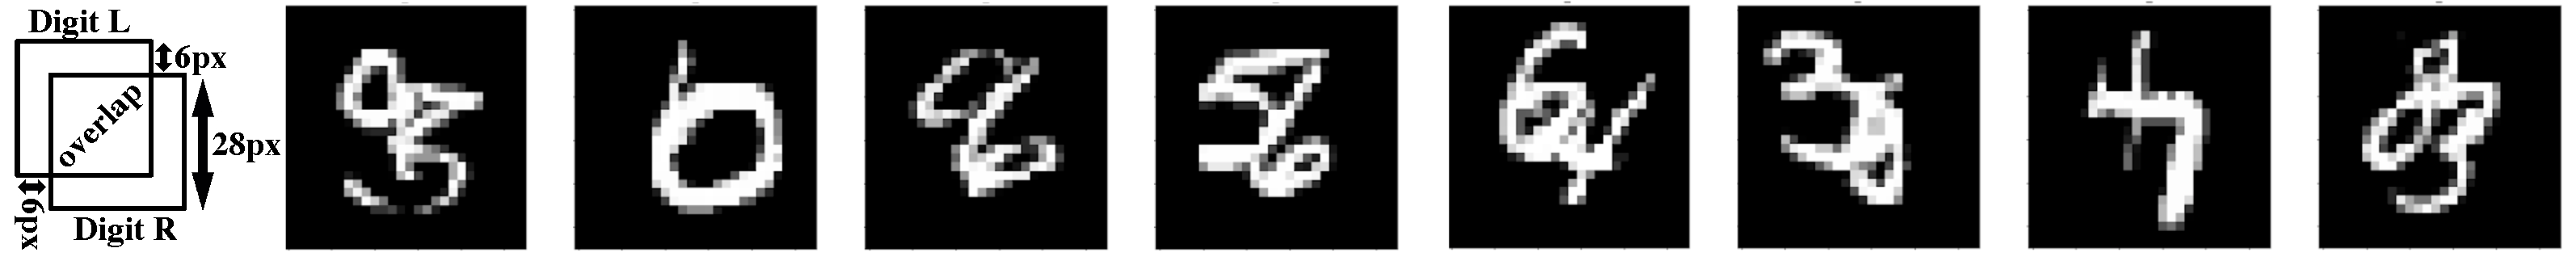
\includegraphics[width=\textwidth]{multi_mnist_vis}
%\captionof{figure}{Visualisation of the image construction for Multi-MNIST, along with randomly sampled examples from the dataset.}
%label{fig:multi_mnist}
%\vspace{5mm}
%\end{figure}%
\begin{tabular}{@{}c@{\hspace{11mm}}c@{}}
\begin{minipage}{.475\textwidth}
  \centering
 % \vspace{-13mm}
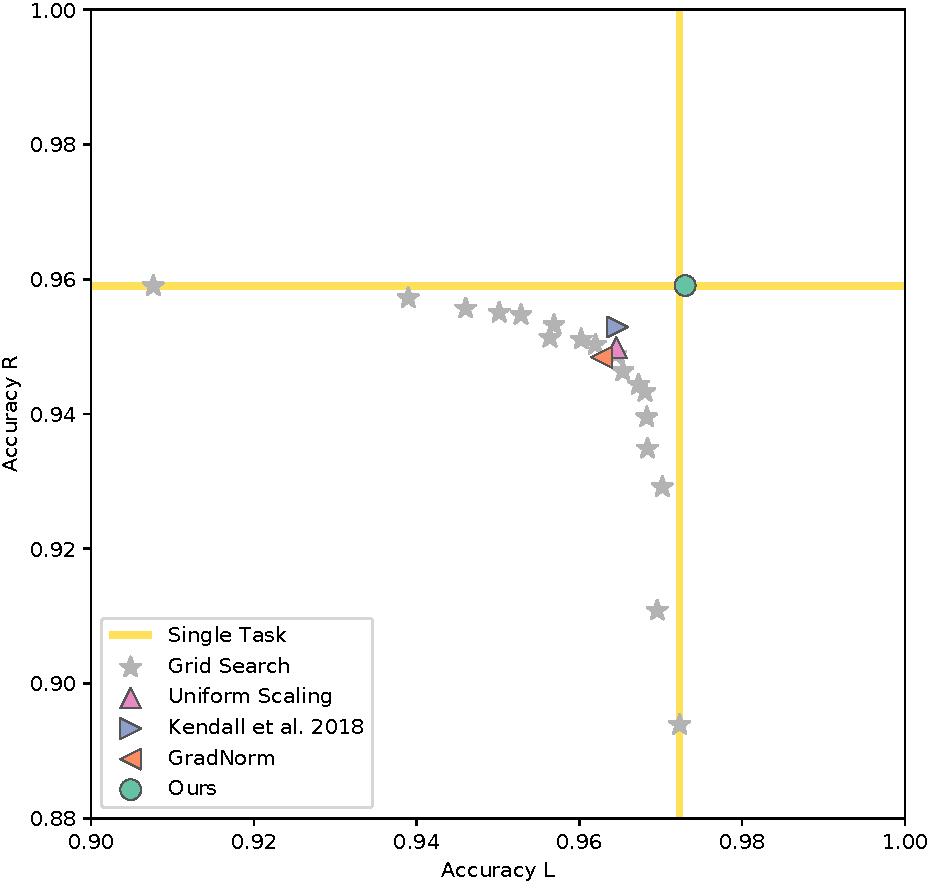
\includegraphics[width=\textwidth]{mnist_left_vs_right}
  \captionof{figure}{\textbf{MultiMNIST accuracy profile.} We plot the obtained accuracy in detecting the left and right digits for all baselines. The grid-search results suggest that the tasks compete for model capacity. Our method is the only one that finds a solution that is as good as training a dedicated model for each task. Top-right is better.}
  \label{fig:multi_mnist_performance_curve}
  \vspace{7mm}
  \captionof{table}{Performance of MTL algorithms on MultiMNIST. Single-task baselines solve tasks separately, with dedicated models, but are shown in the same row for clarity.}
\resizebox{\textwidth}{!}{%
\begin{tabular}{r@{\hspace{4mm}}c@{\hspace{4mm}}c}
\toprule
& Left digit & Right digit   \\
& accuracy [\%] & accuracy [\%]   \\
\midrule
Single task & $\mathbf{97.23}$ & $\mathbf{95.90}$ \\
Uniform scaling & $96.46$ & $94.99$ \\
\citealt{Kendall2018} & $96.47$ & $95.29$ \\
GradNorm & $96.27$ & $94.84$ \\
Ours & $\mathbf{97.26}$ & $\mathbf{95.90}$ \\
\bottomrule
\end{tabular}}
\label{tab:multi_mnist}
  \vspace{7mm}
%\end{minipage}%
%\begin{minipage}{.5\textwidth}
\captionof{table}{Performance of MTL algorithms in joint semantic segmentation, instance segmentation, and depth estimation on Cityscapes. Single-task baselines solve tasks separately but are shown in the same row for clarity.}
\resizebox{\textwidth}{!}{%
\begin{tabular}{r@{\hspace{1mm}}c@{\hspace{2mm}}c@{\hspace{2mm}}c@{}}
\toprule
& Segmentation & Instance & Disparity  \\
& mIoU [\%] &  error [px] &  error [px]  \\
\midrule
Single task & $60.68$ & $11.34$ &  $2.78$\\
Uniform scaling & $54.59$ & $10.38$ & $2.96$ \\
%Grid search & $63.94$  & $5.13$ & $0.562$ \\
\citealt{Kendall2018} & $64.21$ & $11.54$ & $2.65$ \\
 GradNorm  & $64.81$ & $11.31$ & $\mathbf{2.57}$ \\
Ours & $\mathbf{66.63}$ & $\mathbf{10.25}$ & $\mathbf{2.54}$  \\
\bottomrule
\end{tabular}}
\label{tab:cityscapes_results}
%\vspace{-2mm}
\end{minipage}&
\begin{minipage}{.475\textwidth}
  \centering
  \begin{tabular}{@{}r@{}}
  \vspace{1mm} \\
  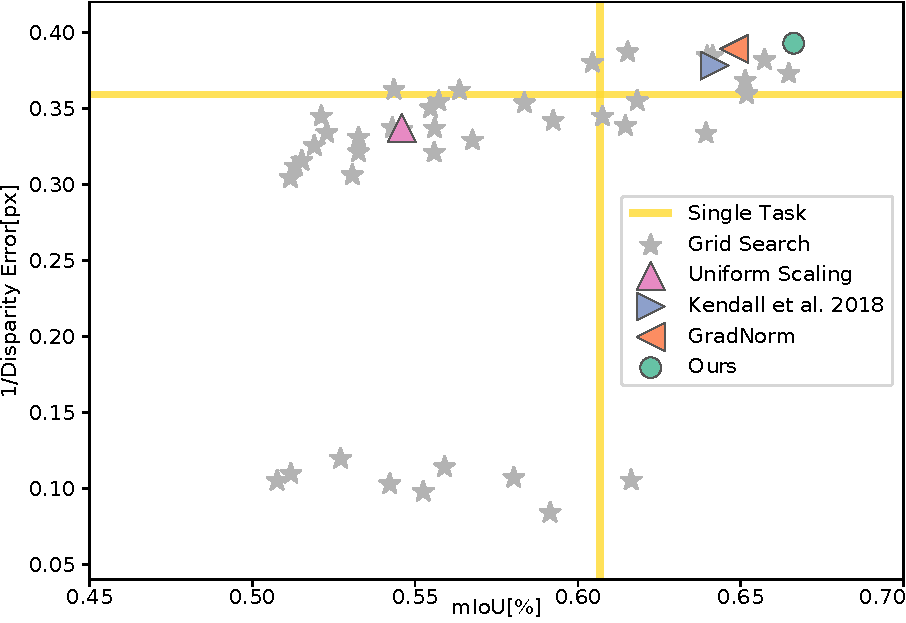
\includegraphics[width=\textwidth]{cityscapes_semantic_depth}   \\ \vspace{2mm} \\
 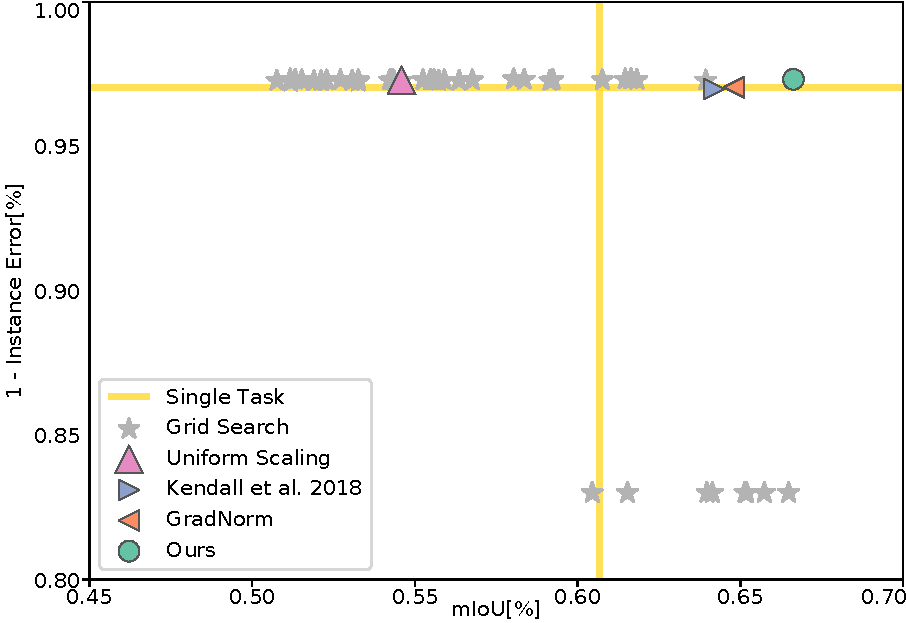
\includegraphics[width=\textwidth]{cityscapes_semantic_instance}  \\ \vspace{2mm} \\
 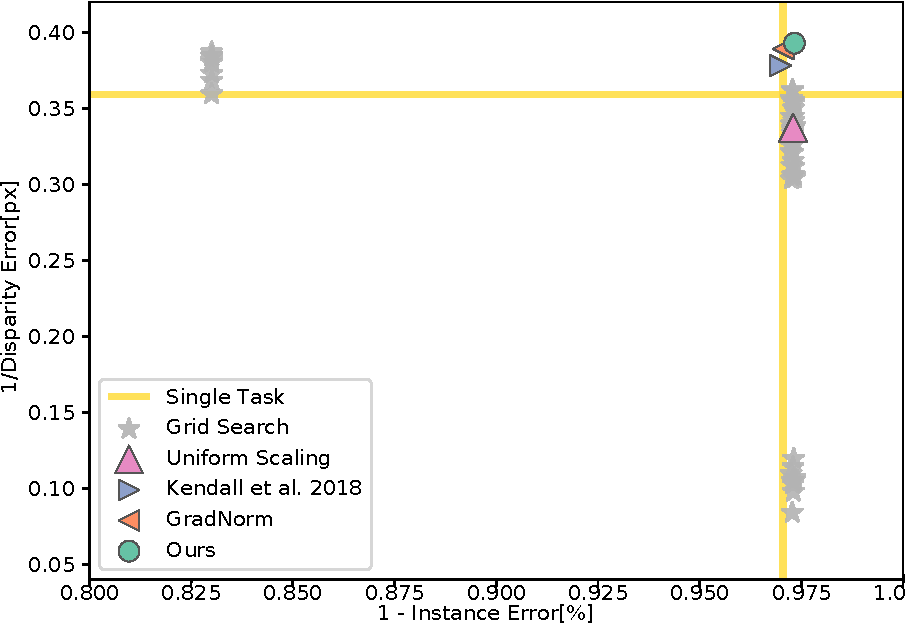
\includegraphics[width=\textwidth]{cityscapes_instance_depth}
\end{tabular}
%\vspace{-2mm}
  \captionof{figure}{\textbf{Cityscapes performance profile.} We plot the performance of all baselines for the tasks of semantic segmentation, instance segmentation, and depth estimation. We use mIoU for semantic segmentation, error of per-pixel regression (normalized to image size) for instance segmentation, and disparity error for depth estimation. To convert errors to performance measures, we use 1 $-$ instance error and 1/disparity error. We plot 2D projections of the performance profile for each pair of tasks. Although we plot pairwise projections for visualization, each point in the plots solves all tasks. Top-right is better.}
  \label{fig:cityscapes_performance_profile}
\end{minipage}%
\end{tabular}
%\vspace{-2mm}
\end{minipage}
